\chapter{Implementace}\label{chap:implementation}

V této kapitole se věnuji implementaci všech navrhnutých komponent, které umožnují automatizaci testování.

\section{Zpráva}
Strukturu jedné zprávy zajišťuje třída \inlinecode{Message}. Digram této třídy můžeme vidět na obrázku \ref{fig:message_class}. Třída \inlinecode{Message} je implementována v jazyce \csharp{} a \cpp{}.

Dle návrhu instance této třídy obsahuje typ zprávy a data zprávy, pokud zpráva nějaké data obsahuje. Typ zprávy je určen enumerátorem \inlinecode{MessageType}. Tento výčtový typ obsahuje jednotlivé typy zpráv, definované v sekci \ref{sec:communication}. Zároveň tyto typy rozšiřuje o hodnotu \inlinecode{MSG\_EXCEPTION}, která značí neplatnou zprávu.

Při odesílání a přijímání zpráv skrz protokol TCP/IP je podstatné, aby se instance třídy dala převádět na bajtové pole a obráceně. Třída \inlinecode{Message} proto obsahuje dvě metody, které tyto převody zajišťují. Tyto metody jsou:

\begin{itemize}
    \item \inlinecode{GetByteStream} -- Metoda převádí instanci třídy \inlinecode{Message} na bajtové pole
    \item \inlinecode{GetMessageFromStream} -- Statická metoda, které v argumentu obdrží bajtové pole a vrátí instanci třídy \inlinecode{Message}.
\end{itemize}

Následná komunikace skrz protokol TCP/IP je implementována v závislosti na zařízení, za pomocí těchto metod. Jednotlivé implementace třídy \inlinecode{Message} mají minimální rozdíly, které jsou primárně kvůli odlišnostem jazyků \csharp{} a \cpp{}.

\begin{figure}[H]
    \centering 
    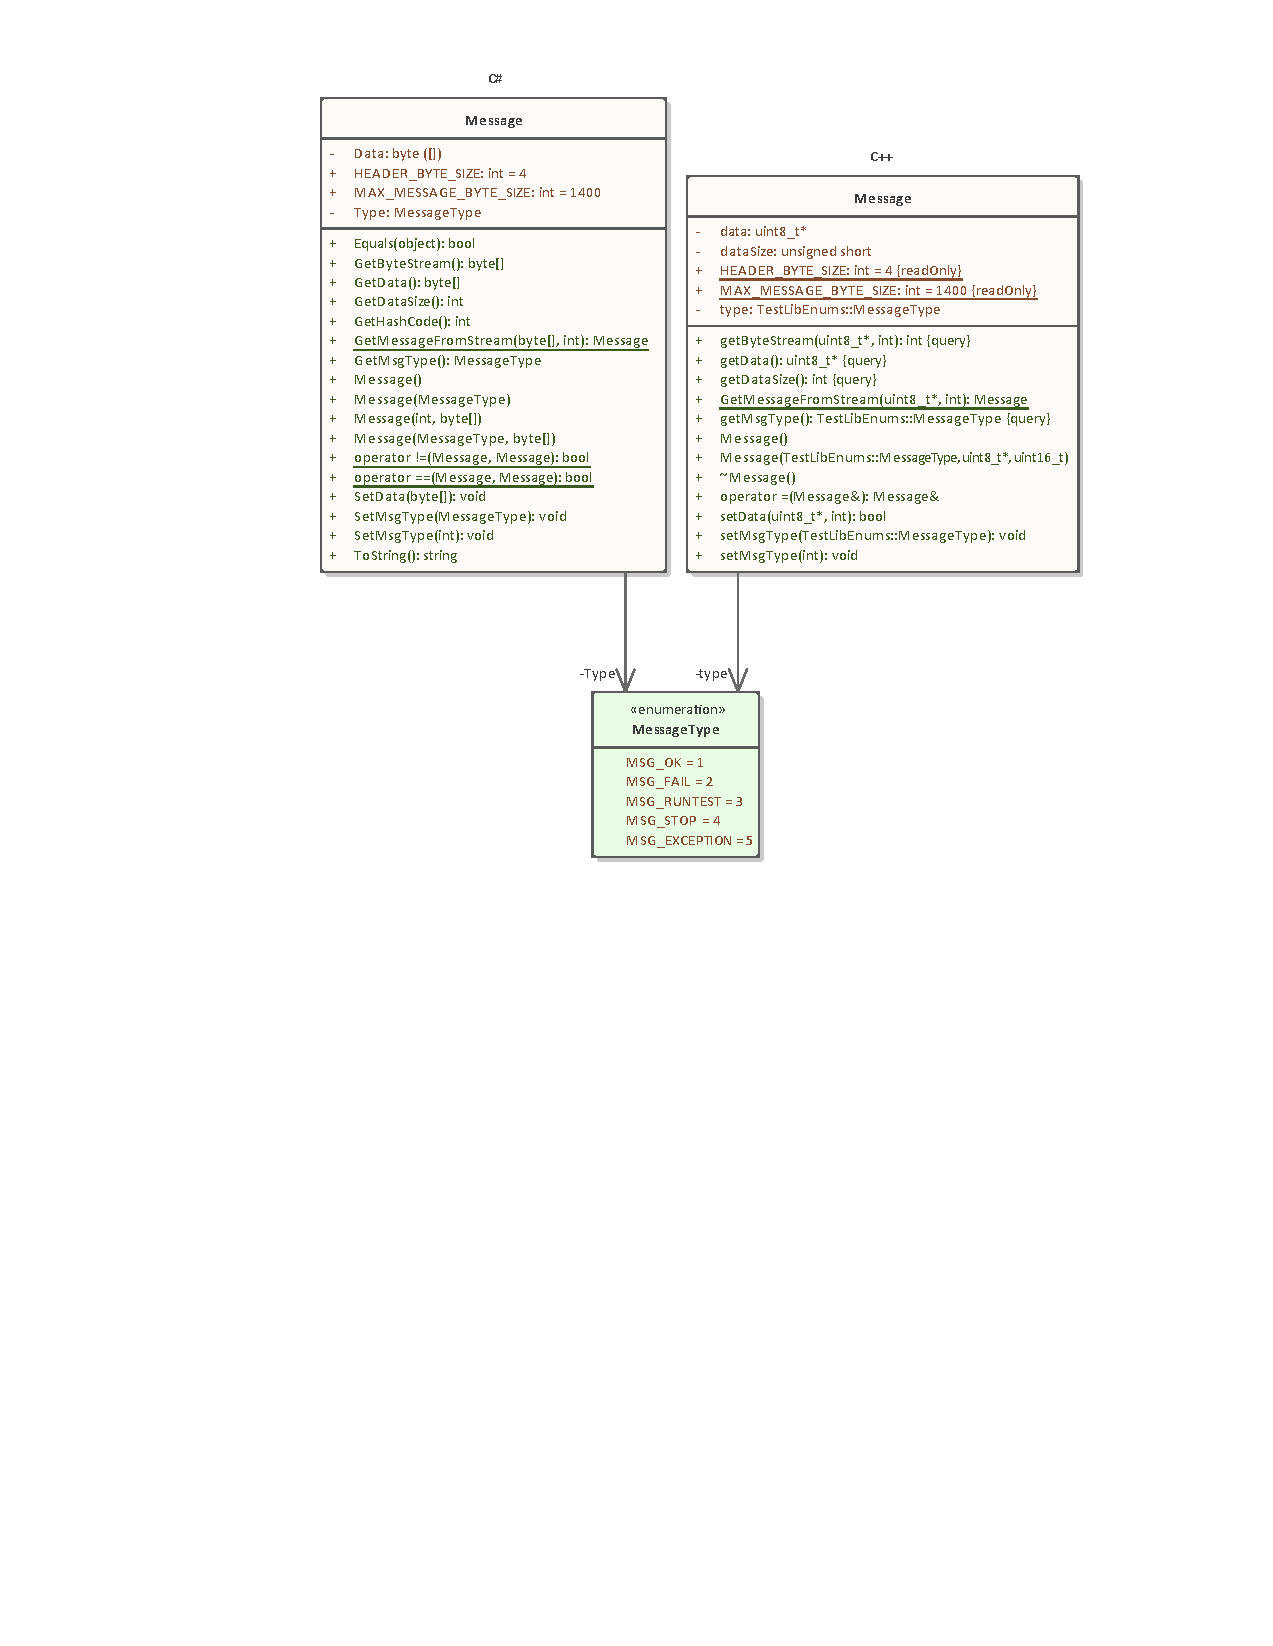
\includegraphics[width=\textwidth]{assets/img/class_diagram/message.pdf}
    \caption{Diagram třídy Message}
    \label{fig:message_class}
\end{figure}

\section{Testovací služba}
Testovací služba je v implementaci rozdělena na dvě hlavní třídy. Třída \inlinecode{TestService} obstarává jednotlivé úkony služby, následně třída \inlinecode{ServiceRunner} propojuje třídu \inlinecode{TestService} s ostatními komponentami, které jsou potřebné pro testování. Tyto třídy můžeme vidět znázorněné na obrázku \ref{fig:test_service}.

\begin{figure}[H]
    \centering 
    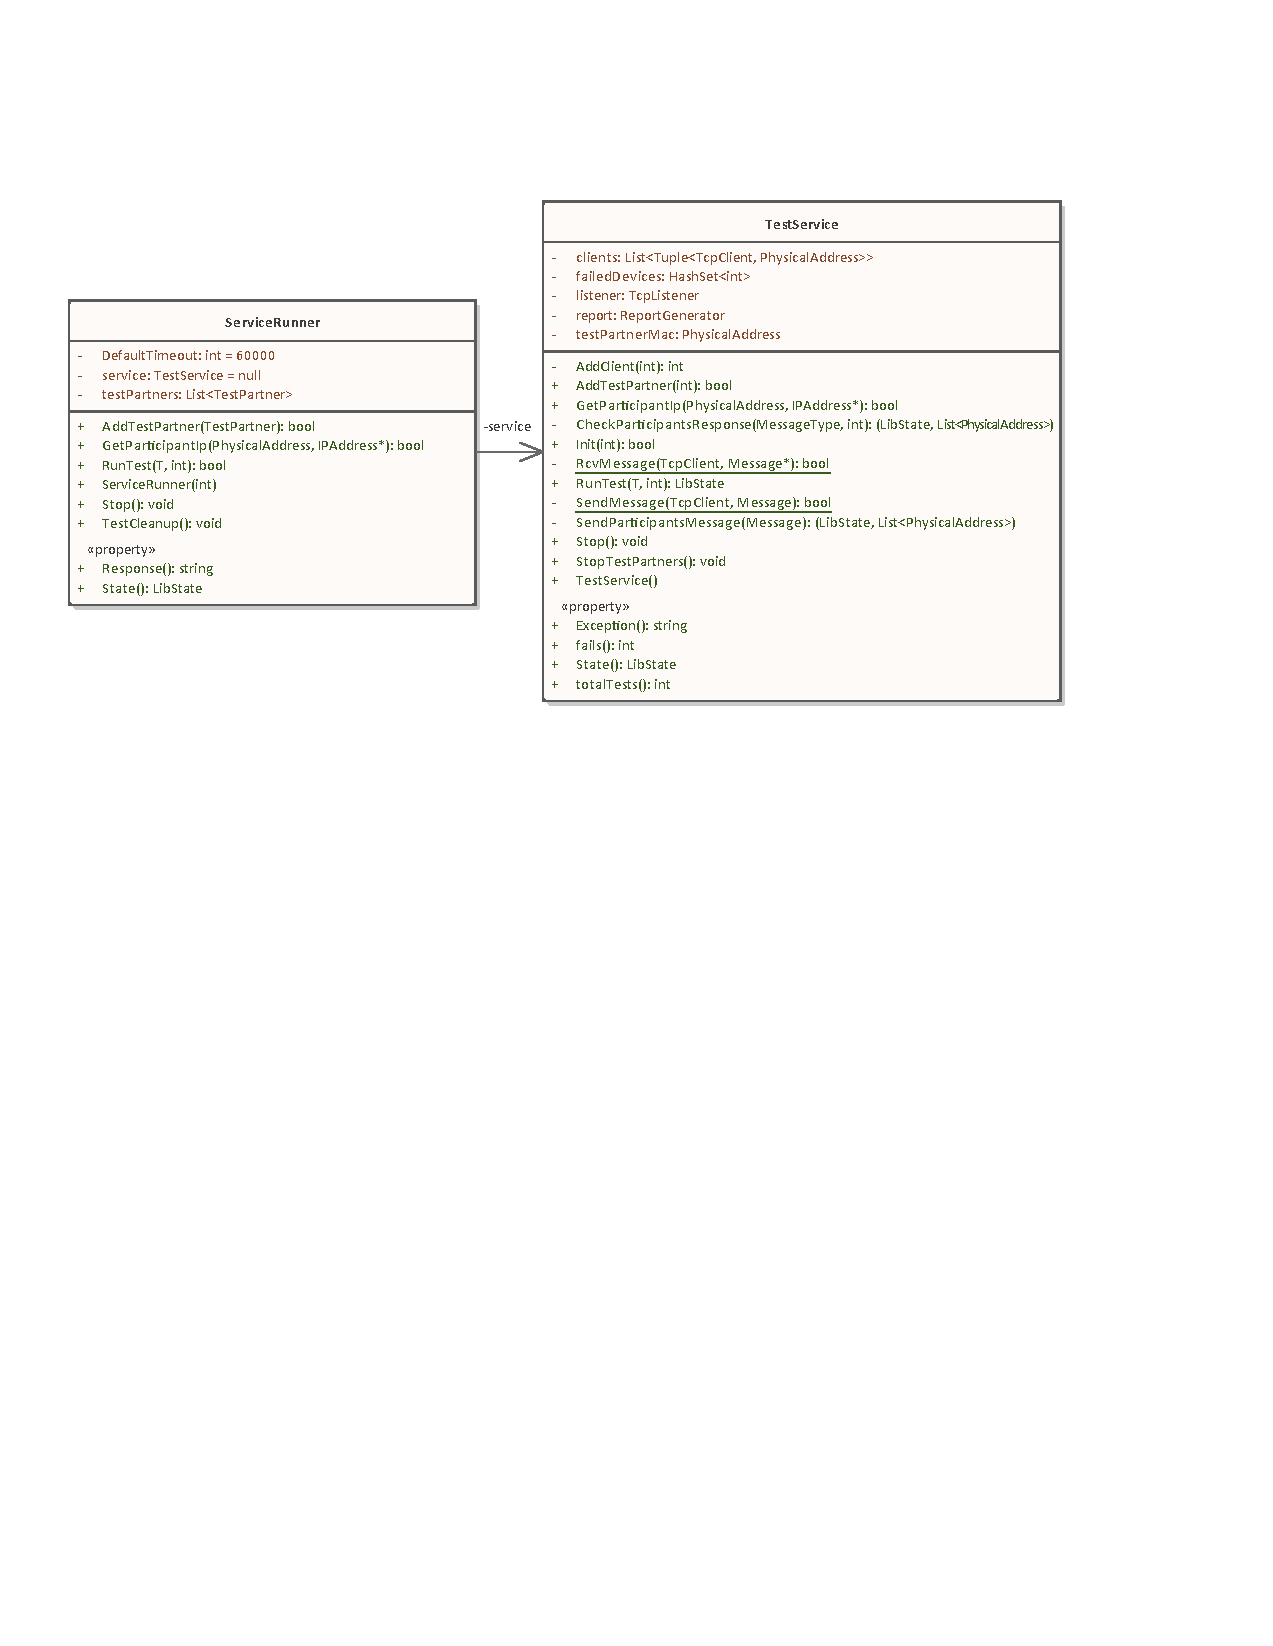
\includegraphics[width=0.90\textwidth]{assets/img/class_diagram/service.pdf}
    \caption{Diagram tříd zajištující testovací službu}
    \label{fig:test_service}
\end{figure}

\subsection{Nastavení služby}\label{sec:settings}

Konfigurace služby je uložena v souboru \inlinecode{config.xml}. Služba očekává tento soubor v kořenové složce, ze které je spouštěna. Tento soubor obsahuje tři hodnoty pro nastavení:

\begin{itemize}
    \item \inlinecode{ip} -- Adresa, na které bude služba poslouchat příchozí připojení. Všechna zařízení se budou připojovat na tuto adresu.
    \item \inlinecode{port} -- Síťový port, skrz který služba provádí komunikaci.
    \item \inlinecode{participants} -- Počet testovaných zařízení, které se připojí ke službě.   
\end{itemize}

Ukázku tohoto souboru můžeme vidět na výpisu \ref{listing:configxml}. V knihovně se o konfiguraci stará třída \inlinecode{Configuration}. Tato třída existuje v jmenném prostoru \inlinecode{GlobalVar}. Tento jmenný prostor simuluje globální proměnnou. Kvůli tomu jsou ale všechny třídy, které jsou odsud používány, konstruovány tak, aby primárně fungovaly jen ke čtení. Zároveň třída \inlinecode{GlobalVar} povolí pouze jedno přiřazení instance. Při pokusu o přiřazení jiné instance třída vyhazuje výjimku. Digram těchto tříd můžeme vidět na obrázku \ref{fig:utility}. Třída také obsahuje vlastnost \inlinecode{isConfigLoaded}, která obsahuje informaci o tom, zdali je konfigurace inicializována.

Při vytvoření instance třída získá konfiguraci z konfiguračního souboru a uloží je do vnitřních proměnných třídy. Tyto proměnné jsou určeny pouze ke čtení, nelze je upravovat. Stav konfigurace určuje proměnná \inlinecode{bool IsValid}. V případě chyby je tato proměnná nastavená na hodnotu \inlinecode{false} a v proměnné \inlinecode{Exception} je uložen důvod neúspěchu. V opačném případě je tato proměnná nastavena na hodnotu \inlinecode{true}.

\begin{listing}[htbp]
    \centering
    \begin{cminted}{xml}
<?xml version="1.0" encoding="UTF-8" ?>
<configuration>
  <!-- IP of the service-->
  <ip>192.168.4.100</ip>
  <!-- Port of the service -->
  <port>1337</port>
  <!-- Number of non-virtualized participants-->
  <participants>1</participants>
</configuration>
    \end{cminted}
    \caption{Ukázka konfiguračního souboru}
    \label{listing:configxml}
\end{listing}


\subsection{Operace služby}

Jak jsem již zmínil, jednotlivé úkony služby jsou implementovány v třídě \inlinecode{TestService}. 
Třída po své konstrukci inicializuje vnitřní proměnné, ale neprovádí žádné úkony. V následujících sekcích přiblížím jednotlivé dostupné operace.

\subsubsection{Odesílání a přijímání zpráv}
Třída \inlinecode{TestService} vytváří během svého běhu propojení s účastníky testování. Po úspěšném připojení služba ke komunikaci používá vestavěného TCP klienta. K této komunikaci má vytvořené dvě statické metody. Tyto metody jsou:

\begin{itemize}
    \item \inlinecode{static void SendMessage(TcpClient client, Message msg)} \\
    Metoda pro odeslání jedné zprávy jednomu klientovi.
    \item \inlinecode{static bool RcvMessage(TcpClient client, out Message msg)} \\
    Metoda pro přijmutí zprávy od jednoho klienta.
\end{itemize}

Všechny zprávy jsou následně odesílány a přijímány za pomoci těchto dvou metod. Rozšířením těchto metod jsou metody:

 {
    \setlength{\emergencystretch}{3em} 
    \begin{itemize}
        \item \inlinecode{(LibState, List<PhysicalAddress>) CheckParticipantsResponse   (MessageType expectedResponse, int timeout)} \\
        Metoda přijme od všech účastníků testování jednu zprávu a zkontroluje je ji s očekávanou zprávou, předanou v argumentu. Zároveň kontroluje, zdali obdrží zprávu v maximálním čase, který je definovaný argumentem \inlinecode{timeout}. 
        \item \inlinecode{(LibState, List<PhysicalAddress>) SendParticipantsMessage (Message msg)} \\
        Metoda odešle všem participantům jednu zprávu.
    \end{itemize}
 }

Obě zmíněné metody následně v návratové hodně vrací dvě položky. První položkou je výsledek operace. Tento výsledek je reprezentován enumerátorem \inlinecode{LibState}. Tento enumerátor má tyto výčty:

\begin{itemize}
    \item \inlinecode{STATE\_OK} - označuje úspěch
    \item \inlinecode{STATE\_FAIL} - označuje neúspěch
    \item \inlinecode{STATE\_ERROR} - označuje fatální neúspěch, jehož důvodem je nějaká chyba
\end{itemize}

Tento enumerátor je zároveň hojně využíván skrz knihovnu k reprezentaci stavu různých komponent. Druhou položkou, kterou metoda vrací, je seznam zařízení, které se při komunikaci způsobily neúspěch. Tento neúspěch může vzniknout ať už obdržením jiné zprávy než očekávané v případě metody \inlinecode{CheckParticipantsResponse}, a nebo vznikem nějaké chyby při komunikaci.

\subsubsection{Inicializace}

Třída \inlinecode{TestService} pro účely inicializace a přidání klienta má tyto dvě metody:

\begin{itemize}
    \item \inlinecode{bool Init(int InitTimeout)} \\
    Metoda, která provádí inicializační fázi testovací služba
    \item \inlinecode{int AddClient(int timeout)}\\
    Metoda pro přidání klienta do testovací služby
\end{itemize}

Metodou \inlinecode{Init} třída inicializuje běh služby. Metoda z konfigurace zjistí IP adresu a port, na kterém má služba běžet. Následně začne na této IP adrese a portu poslouchat příchozí komunikaci. Z nastavení služba ví, kolik připojení má očekávat. 

Proměnná \inlinecode{InitTimeout} určuje dobu, kdy služba čeká na příchozí komunikaci. Doba je metodě předávána, stejně jako všem ostatním metodám, které mají definovaný časový limit, v milisekundách. Metoda synchronně kontroluje, zdali nějaký účastník nečeká na připojení a zdali nevypršela maximální doba na připojení. V případě příchozí komunikace metoda zavolá metodu \inlinecode{AddClient}. Pokud se chce v jeden moment připojit více účastníků, tak ostatní účastníci jsou zařazeni do fronty.

Po zavolaní metody \inlinecode{AddClient} metoda vytvoří připojení s testovacím zařízením a následně čeká na identifikační zprávu od testovacího zařízení, nejdéle avšak čeká po dobu definovanou argumentem \inlinecode{timeout}. 

Po obdržení zprávy metoda uloží vytvořeného klienta a jeho MAC adresu do seznamu připojených účastníků testování. Nakonec metoda vrací tři hodnoty typu integer:
\begin{itemize}
    \item \inlinecode{0} -- pokud připojení účastníka testování vyústilo v neúspěch, ať už kvůli překročení časového limitu, nebo kvůli nedodržení stanovené komunikace
    \item \inlinecode{1} -- pokud se ke službě úspěšně připojí testované zařízení
    \item \inlinecode{2} -- pokud se ke službě úspěšně připojí testovací partner
\end{itemize}

Metoda \inlinecode{AddClient} za testovacího partnera takového účastníka, který odešle jako svoji MAC adresu testovacího partner. Zařízení, která odešlou jinou MAC adresu jsou považována jako testovaná zařízení. Metoda považuje nulovou MAC adresu jako neplatnou.

Služba úspěšně ukončuje inicializační fázi poté, co se úspěšně připojí stejný počet účastníků testovaní, jako bylo určeno v konfiguraci. V případě nepřipojení se očekávaného počtu zařízení v definovaném čase, obdržení špatné nebo žádné zprávy služba vyhodnocuje inicializační fázi jako neúspěšnou. Připojení testovacího partnera v této fázi vyústí též v neúspěch inicializace. 

\subsubsection{Připojení testovacího partnera}

Jelikož každý test může obsahovat různý počet testovacích partnerů, je podstatné, aby služba mohla při testovacím běhu tyto zařízení přidávat a odebírat. K tomuto slouží dvě metody. Metoda \inlinecode{AddTestPartner} řekne službě, že má očekávat připojení testovacího partnera. V případě úspěšného připojení metoda vrací úspěch. Naopak v případě chyby, nebo připojení jiného zařízení, metoda vrací neúspěch. O opačnou operaci se stará metoda \inlinecode{StopTestPartners}. Metoda po svém zavolání odešle všem testovací partnerům zprávu o ukončení testování a tato zařízení jsou odpojena a ukončena.

\subsubsection{Spuštění testu}

Nejpodstatnější operací je spuštění jednotlivých testů. O toto se stará metoda \inlinecode{LibState RunTest<T>(T testEnum, int timeout)}. Metoda očekává dva parametry:

\begin{itemize}
    \item \inlinecode{T testEnum} -- Identifikátor testu s generickým typem T, který typem musí být enumerátor.
    \item \inlinecode{int timeout} -- Maximální délka, po kterou služba očekává odpověď od účastníků testu. 
\end{itemize}

Metoda odesílá všem účastníkům testování direktivu k započnutí jednotlivých fází testu. Následně poté čeká na odpověď od všech účastníků testu. Doba čekání je určena argumentem \inlinecode{timeout}. Tento čas je vázaný na jednotlivá stádia testování. Tedy pokud metoda má časový limit 30 sekund, tak poté bude po každém odeslání direktivy k započnutí fáze testu čekat na odpověď maximálně těchto stanovených 30 sekund. Tento časový limit je realizován za pomoci metody \inlinecode{CheckParticipantsResponse}.

Metoda během běhu vyhodnocuje, zda se účastníka testování nedostal do chybové stavu. Na základě toho poté spouští jednotlivé fáze. Po skončení testu metoda vrací jednu z hodnot enumerátoru \inlinecode{LibState}. 

\subsubsection{Ukončení testování}

Po dokončení celého testovacího běhu je zavolána metoda \inlinecode{Stop()}. Tato metoda odešle všem stále připojeným účastníkům direktivu k ukončení testování a ukončí spojení. Služba se snaží v případě chyby ukončit co nejvíce zařízení skrz stanovený protokol.

\subsubsection{Pomocné třídy}
Třída \inlinecode{TestService} využívá dvě pomocné třídy při svém běhu, jejichž diagram můžeme vidět na obrázku \ref{fig:utility}. První třídou je třída \inlinecode{Logger}. Tato třída realizuje zapisování protokolu do souboru během běhu. Zároveň zapisovat může maximálně jedno vlákno současně. Třída je obsažena taktéž ve třídě \inlinecode{GlobalVar}, která simuluje globální proměnnou. Inicializace instance třídy \inlinecode{Logger} lze provést odkudkoliv, avšak stejně jako u konfigurace pouze jen jednou. Třída \inlinecode{GlobalVar} obsahuje vlastnost \inlinecode{isLogEnabled}, která obsahuje informaci o tom, zdali je zapisování inicializováno.  

Třída \inlinecode{TestService} obsahuje ve svých metodách kontrolu, zdali je instance třídy \inlinecode{Logger} inicializována a v případě kladného vyhodnocení zapisuje průběh svého běhu. Instance třídy \inlinecode{Logger} by teda měla být vytvořena ještě před započnutím běhu služby.

Druhou třídou, kterou třída \inlinecode{TestService} využívá, je třída \inlinecode{ReportGenerator}. Tato třída vytváří výstupní XML soubor s výsledky jednotlivých testů.
Tento soubor je vytvořen ve formátu dle frameworku NUNit, jehož definici můžeme najít v \cite{nunit}. Tento soubor následně může být nahrán do serveru Azure DevOps. V navrhnutém řešení je tento výstup považován jako záložní.

\begin{figure}[htbp]
    \centering 
    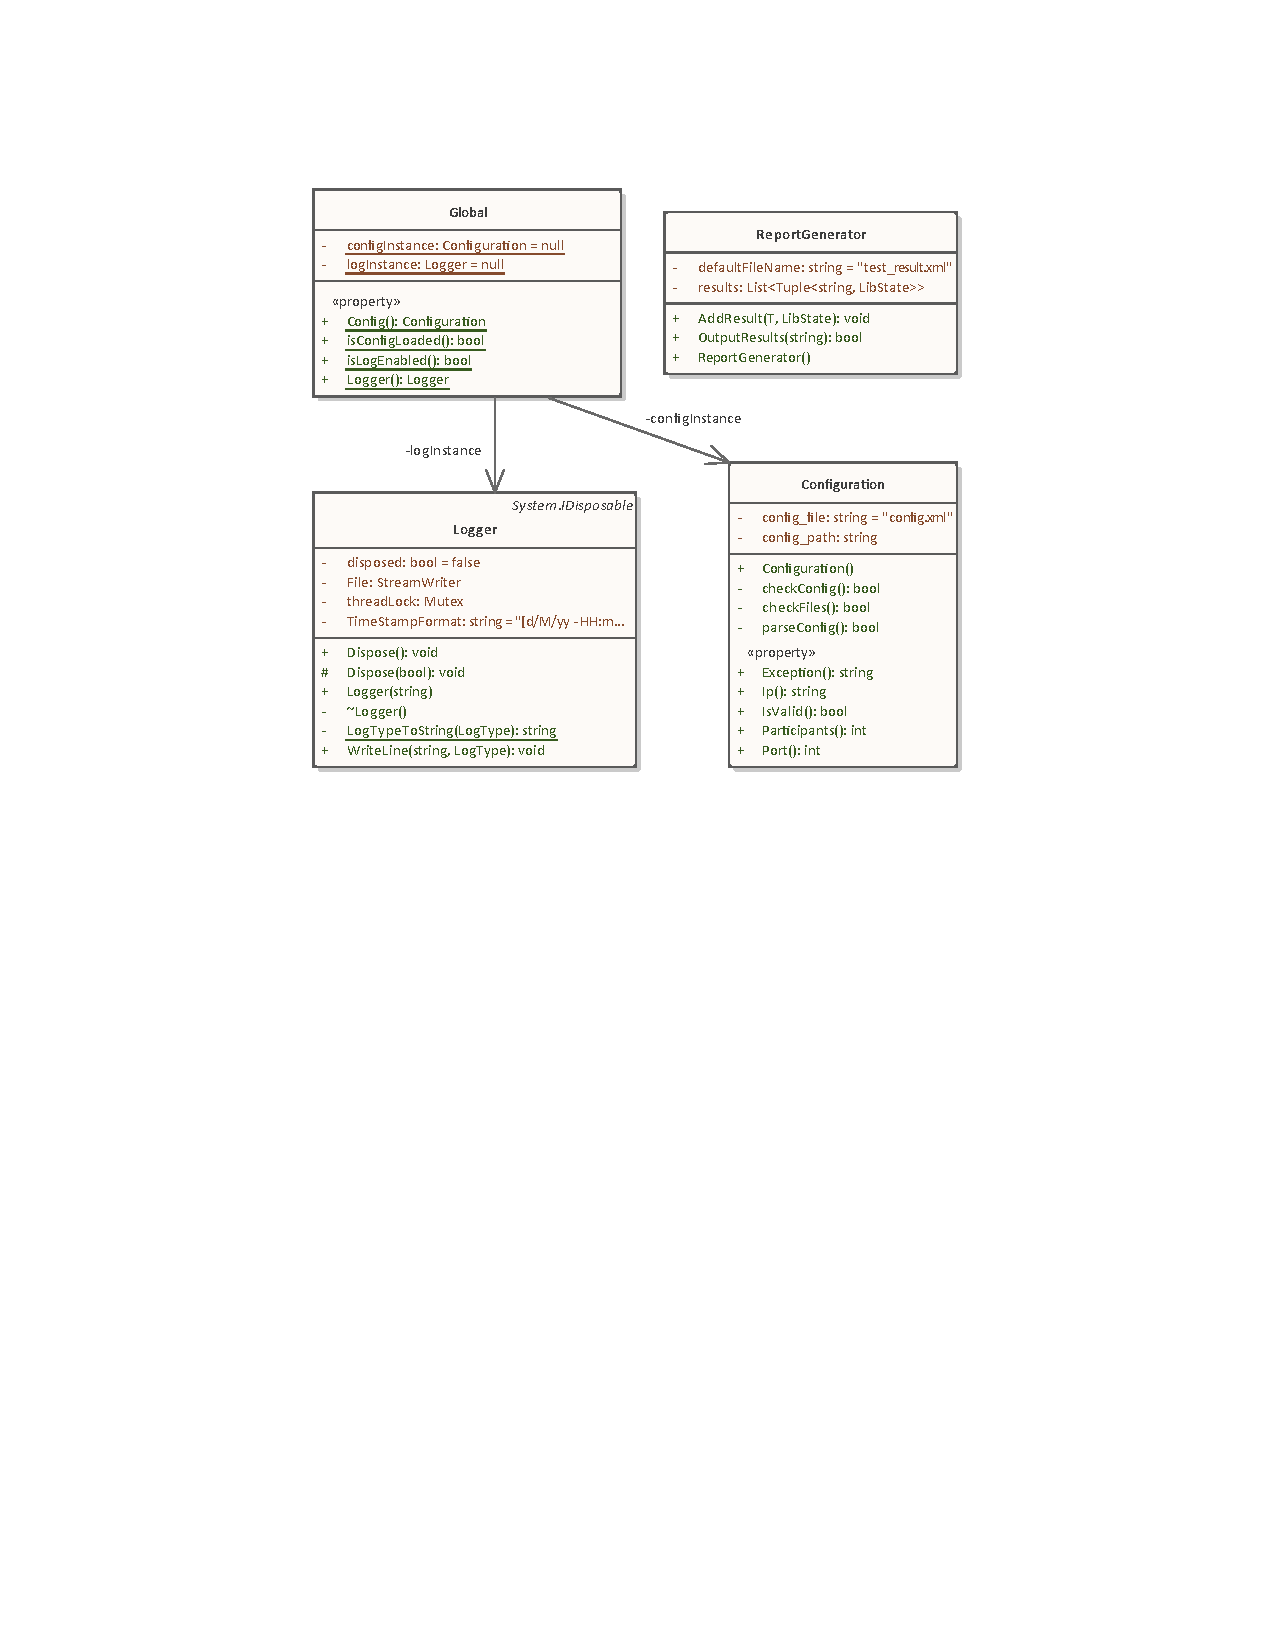
\includegraphics[width=\textwidth]{assets/img/class_diagram/utility.pdf}
    \caption{Diagram tříd, které zajišťují pomocné služby}
    \label{fig:utility}
\end{figure}


\subsection{Propojení s ostatními komponentami}

O propojení třídy \inlinecode{TestService} s ostatními komponentami knihovny se stará třída \inlinecode{ServiceRunner}.
Tato třída ve svém konstruktoru inicializuje konfiguraci služby a zjistí, zda je validní. Tento konstruktor přijímá jeden argument -- časový limit na inicializaci. V případě nezadání tohoto parametru třída využije defaultní časový limit definovaný ve třídě na 60 sekund. Následně konstruktor vytvoří instanci třídy \inlinecode{TestService} a zavolá metodu \inlinecode{Init}. V případě jakékoliv chyby je služba vyhodnocena jako v chybovém stavu. Toto určuje enumerátor \inlinecode{LibState} v proměnné \inlinecode{State}. Třída využívá pouze hodnoty \inlinecode{STATE\_OK} a \inlinecode{STATE\_ERROR}. Následný důvod vyhodnocení chyby je uloženo v proměnné \inlinecode{Response}. Třída následně má další metody, skrz které umožňuje ovládání instance třídy \inlinecode{TestService}. Tyto metody jsou:

\begin{itemize}
    \item \inlinecode{bool RunTest<T>(T test, int timeout = DefaultTimeout)} \\ Metoda předá instrukci pro spuštění testu. Očekává stejné parametry jako metoda \inlinecode{RunTest} třídy \inlinecode{TestService}. Jedinou změnou je, že pokud časový limit nebude zadán, tak bude použit defaultní časový limit.
    \item \inlinecode{bool AddTestPartner(TestPartner participant)} \\ Metoda spouští testovacího partnera předaného v argumentu a předává informaci o očekávání jeho připojení  instanci třídy \inlinecode{TestService}. Instanci partnera následně uloží.
    \item \inlinecode{void TestCleanup()} \\ Metoda je volána po dokončení jednotlivého testu. Metoda předá instanci třídy \inlinecode{TestService} direktivu k odpojení testovacích partnerů. Následně zkontroluje, zda se partneři ukončily a pokud ne, tak partnery ukončí.
    \item \inlinecode{void Stop()} \\ Metoda předá informaci o ukončení testovacího běhu.
\end{itemize}

\section{Rozhraní pro testovaná zařízení}\label{sec:testrunner}

Diagram tříd, které realizují implementaci pro účastníka testování, můžeme pro implementaci v jazyku \cpp{} vidět na obrázku \ref{fig:test_client_cpp} a pro implementaci v jazyku \csharp{} na obrázku \ref{fig:test_client_csharp}. Obě implementace obsahují rozhraní pro testované zařízení, které je následně na testovaném zařízení implementováno testerem.

Vytvořené rozhraní je následně využito ve třídě \inlinecode{TestRunner}. Tato třída zajištuje běh jednotlivých účastníků testování. Třída je rovněž implementována v jazycích \csharp{} a \cpp{}. Třída obsahuje tyto metody: 

\begin{itemize}
    \item \inlinecode{Init(ipAddress,port)} \\ Metoda inicializuje připojení s testovací službou, kde parametry připojení k službě jsou obdrženy v argumentech funkce.
    \item \inlinecode{HandleInstructions()} \\ Metoda přijímá instrukce od testovací služby a na základě nich provádí úkony.
    \item \inlinecode{RunTest(testIdentifier, testState)} \\ Metoda spouští jednotlivé fáze testů. 
    \item \inlinecode{Stop()} \\ Metoda ukončuje testovací běh.
\end{itemize}

Bližší vysvětlení si zaslouží metoda \inlinecode{RunTest}. Tato metoda je volána z metody \inlinecode{HandleInstruction}. K udržení stádia testu si třída mezi jednotlivými stádii drží instanci jednotlivých testů. Ve fázi přípravy na testování metoda zkontroluje že instance testu je nastavena na hodnotu \inlinecode{null}. Jiná hodnota by značila chybu během předchozího testování. Ve fázi úklidu po dokončení testu je odkaz na instanci testu nastaven na zpátky hodnotu null. Třída \inlinecode{TestRunner} je opět implementována v jazyce \csharp{} a \cpp{}.

Návrhově je jak rozhraní pro zařízení, tak třída \inlinecode{TestRunner} v obou implementacích ekvivalentní. Je třeba ale upřesnit implementaci v \cpp{}. Tato implementace je mířena na testované zařízení, které běží na vlastním speciálně vyvinutém hardwaru. Zařízení avšak v některých případech nepoužívá některé vestavěné funkce a místo nich používá jejich vlastní náhradu. 

Implementace v \cpp{} tedy definuje seznam funkcí, které jsou potřeba implementovat, resp. je potřeba u nich vytvořit odkaz na funkce, které jsou implementované na zařízení. Seznam těchto funkcí můžeme vidět na výpisu \ref{listing:cppinterface}. Z tohoto výpisu lze vidět, že to jsou funkce, které alokují a uvolňují paměť na haldě, a funkce, která paměť kopíruje. 

\begin{listing}[H]
    \centering
    \begin{minted}[breaklines]{cpp}
/*  Allocation of memory on heap 
 */
void* TESTLIB_ALLOC_MEM( const uint32_t length );

/* Free of allocated memory 
 */
bool TESTLIB_FREE_MEM(void* ptr);

/* Copy of memory 
 */
void* TESTLIB_MEMCPY(void* const lpDst, const void* const lpSrc, int dwNb);
    \end{minted}
    \caption{Seznam funkcí k implementaci na zařízení v jazyce \protect\cpp{}}
    \label{listing:cppinterface}
\end{listing}


\section{Testovací partner}
Implementace testovacího partnera přímo kopíruje navrhnuté rozhraní pro testované zařízení. Jeho logika je obsažena ve třídě \inlinecode{TestPartner}. Diagram třídy můžeme vidět také na obrázku \ref{fig:test_client_csharp}. Tato třída má tři možné konstruktory:

\begin{itemize} 
    \item \inlinecode{TestPartner(ITestClient device)} \\
    Konstruktor dostane v argumentu odkaz na instanci rozhraní zařízení.
    \item \inlinecode{TestPartner (ITestCase testCase)} \\
    Konstruktor dostane v argumentu odkaz na instanci jednoho testu, který je odvozený z rozhraní pro test.
    \item \inlinecode{TestPartner (Func<UInt32, ITestCase> getTest)} \\
    Argumentem konstruktoru je funkce, která obsahuje seznam testů. Funkce v argumentu dostane číselnou reprezentaci testu a vrací instanci testu, který je odvozený z rozhraní testu.
\end{itemize}

Třída následně vytvoří instanci implementovaného rozhraní pro zařízení (třída \inlinecode{PartnerDevice}), který přijme v konstruktoru vybraný způsob reprezentace testů. Instanci rozhraní následně předá instanci třídy \inlinecode{TestRunner} a po zavolání metody \inlinecode{Start} spustí instanci třídy \inlinecode{TestRunner} na vlastním vlákně.

Třída také obsahuje metodu \inlinecode{Stop}, která po zavolání kontroluje ukončení testovacího partnera v daném časovém limitu. Po vypršení časového limitu funkce ukončuje vlákno, na kterém instance třídy \inlinecode{TestRunner} běží.

\begin{figure}[H]
    \centering 
    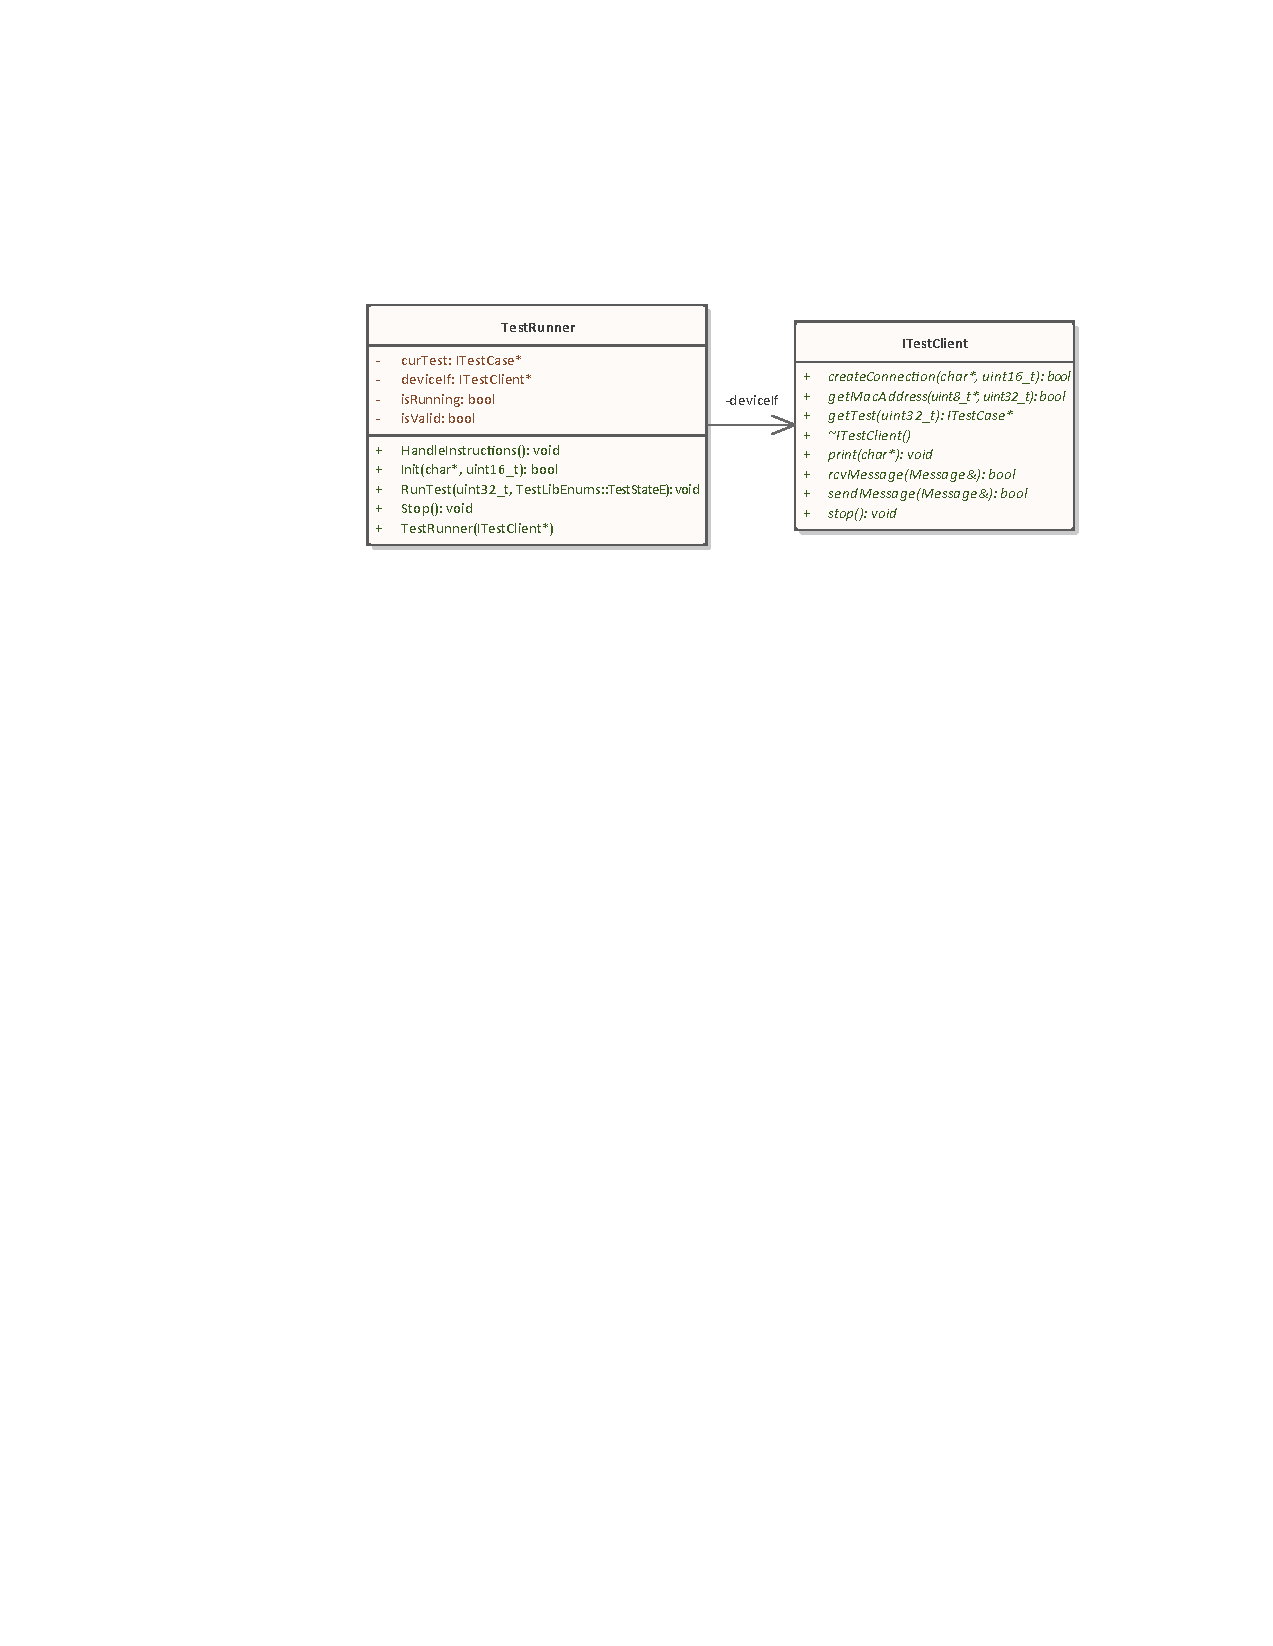
\includegraphics[width=\textwidth]{assets/img/class_diagram/client-cpp.pdf}
    \caption{Diagram tříd implementace účastníka testování v jazyce \protect\cpp{}}
    \label{fig:test_client_cpp}
\end{figure}

\begin{figure}[H]
    \centering 
    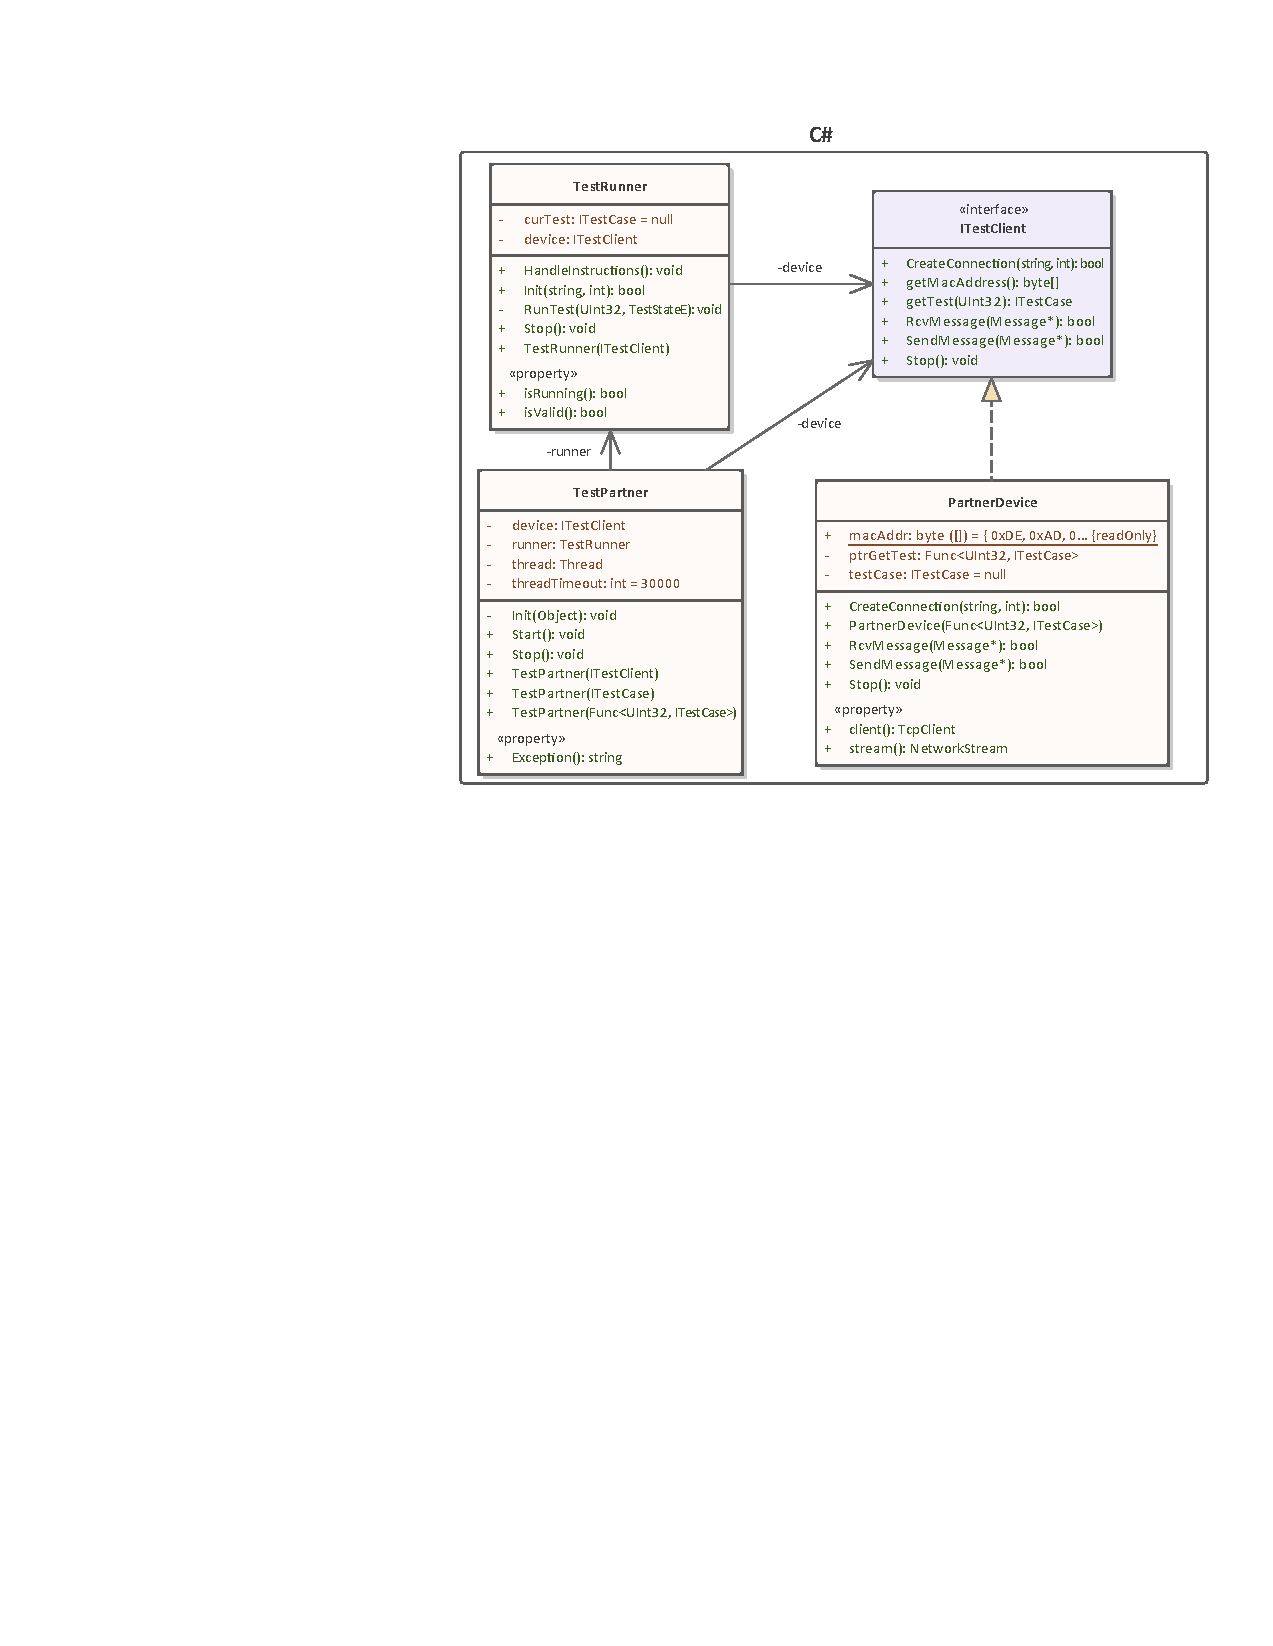
\includegraphics[width=\textwidth]{assets/img/class_diagram/client-csharp.pdf}
    \caption{Diagram tříd implementace účastníka testování v jazyce \protect\csharp{}}
    \label{fig:test_client_csharp}
\end{figure}


\section{Propojení s frameworkem MSTest}

Podstatnou součástí implementace je propojení služby s testovacím frameworkem MSTest. O toto se stará třída \inlinecode{API}. Jako jediná třída využívá nástroje tohoto frameworku. Třída je koncipovaná jako statická třída, i když je závislá na jím vytvořené instanci třídy \inlinecode{ServiceRunner}. Toto je uděláno kvůli kompatibilitě s frameworkem MSTest. 


\subsection{Použití frameworku}
Jak jsem již zmínil v sekci \ref{sec:reg_test_design}, framework MSTest pro identifikaci testových metody využívá atributy. Framework MSTest využívá například tyto atributy:

\begin{itemize}
    \item \inlinecode{AssemblyInitialize} -- identifikuje inicializační funkci, která je spuštěna před spuštěním testů \cite{attr_init_clean}
    \item \inlinecode{AssemblyCleanup} -- identifikuje funkci která bude spuštěna po skončení všech testů \cite{attr_init_clean}
    \item \inlinecode{TestClass} -- identifikuje třídu, která obsahuje testy \cite{mstest_docs}
    \item \inlinecode{TestMethod} -- identifikuje metody, které reprezentují jednotlivé  testy \cite{mstest_docs}
\end{itemize}

Framework MSTest následně používá tyto metody, které jsou identifikovány těmito a dalšími atributy. Při kompilaci jazyk \csharp{} vytváří jednotlivé celky kompilovaného kódu, které poté spojuje do logického celku. Tyto jednotlivé celky se nazývají \textit{assembly}. \cite{assembly}

Implementace testovací knihovny a uživatelské použití knihovny, a tedy i testovacího frameworku MSTest, tvoří samostatné logické celky. Framework MSTest následně detekuje správně definované funkce pouze z toho logického celku, ze kterého je spouštěn.

\subsection{Spuštění a ukončení služby}

Při spuštění jednotlivých testů je nutné brát v potaz, že testovací služba neví jaké testy budou kdy spuštěny. Testovací služba se tedy musí používat nezávisle na všech testech. K tomuto využijeme dvě funkce frameworku MSTest -- \inlinecode{AssemblyInitialize} a \inlinecode{AssemblyCleanup}. Tyto dvě funkce jsou spuštěny ještě před započnutím a po skončení testovaní. V třídě \inlinecode{API} jejím implementacím odpovídají metody \inlinecode{AssemblyInit} a \inlinecode{AssemblyCleanup}. Metoda \inlinecode{AssemblyInit} přijímá dva argumenty:

\begin{itemize}
    \item \inlinecode{Assembly assembly} -- odkaz na runtime blok, který odkazuje na uživatelskou část použití testovací knihovny
    \item \inlinecode{int InitTimeout} -- časový limit na inicializační fázi služby (tedy časový limit, který je využíván v metodě \inlinecode{TestService.Init}), pokud je ponechán prázdný, je použit defaultní časový limit z třídy \inlinecode{ServiceRunner}.
\end{itemize}

Metoda \inlinecode{AssemblyInit} na počátku kontroluje kolize mezi testovými identifikátory. Způsob kontroly je popsán v sekci \ref{sec:reg_test_impl}. Metoda následně inicializuje službu, která projde inicializační fází. 

Metoda \inlinecode{AssemblyCleanup} symetricky ukončuje běh testovací služby. V určitých případech tato funkce nemusí být zavolána. Při zjištění chyby v běhu, která vyústí v ukončení testovacího běhu, je tedy tato funkce zavolána manuálně. Zároveň je kontrolováno, aby tato metoda nebyla volána vícekrát.

Aby mohl MSTest rozeznat tyto funkce, je potřeba je definovat ve stejné assembly, která spouští tento framework. Toto vytváří problém u automatizace vytvoření propojení s testovací knihovnou. Pokud v testovací knihovně definujeme metody, které budou obsahovat atributy \inlinecode{AssemblyInitialize} a \inlinecode{AssemblyCleanup}, tak testovací framework  MSTest tyto metody nevidí a tím pádem je nepoužije. Proto je potřeba vytvořit dvě funkce, které budou obalovat metody \inlinecode{AssemblyInit} a \inlinecode{AssemblyCleanup}, ve stejné assembly, jako ve které běží framework MSTest.

Toto zpravuje třída \inlinecode{TestLibInit}. Tato statická třída pouze zaobaluje tyto dvě metody svými metodami a přidává k nim potřebné atributy. Tato třída není součásti assembly testovací knihovny. V kontextu samotné knihovny je to pouze textový soubor. Proces propojení této třídy s testovacím projektem, ve kterém poběží framework MSTest, je popsán v sekci \ref{sec:distrbution}.

\subsection{Registrování testů}\label{sec:reg_test_impl}

Při rozlišování jednotlivých testů knihovna a testovací služba využívá enumerátory. Tyto enumerátory odkazují na nějakou číselnou hodnotu, které je následně odesílána testovaným zařízením. Všechny enumerátory musí být označeny atributem \inlinecode{TestEnum}. Díky němu může knihovna identifikovat výčtové typy, které reprezentují testy a zjistit mezi nimi kolize. 

Tato kontrola je provedena před započnutím testování v metodě \inlinecode{AssemblyInit} díky odkazu na runtime blok, který obdrží v argumentu. Tato kontrola se dá přeskočit předáním hodnoty \inlinecode{null} jako odkazu na na runtime blok.

Framework MSTest registruje testy nezávisle na testovací knihovně. Jednotlivé třídy musí být označený atributem \inlinecode{TestClass} a zároveň jednotlivé metody atributem \inlinecode{TestMethod}. Framework následně testy detekuje automaticky.

\subsection{Spuštění testu}
Pro spuštění testu je použita metoda \inlinecode{Run} z třídy \inlinecode{API}. Tato metoda přijímá stejné argumenty jako metoda \inlinecode{RunTest} třídy \inlinecode{ServiceRunner}. Metoda zkontroluje, že argument identifikující test je typem enumerátor a obsahuje atribut \inlinecode{TestEnum}. V případě že se testovací služba nenachází v chybném stavu, tak metoda předá testovací službě direktivu k započnutí testu. Následně vyhodnotí úspěšnost testu. V případě, že služba je v chybném stavu, metoda vyhodnotí test jako bezvýsledný.

Zároveň lze před započnutím testu přidat testovací partnery. Toto je možné za pomocí metody \inlinecode{AddTestPartner} z třídy \inlinecode{API}. Metoda v argumentu obdrží instanci testovacího partnera a následně se postará o běh tohoto participanta.


\section{Vytvoření balíčku NuGeT a distribuce knihovny}\label{sec:distrbution}

Knihovna je distribuována jako NuGet balíček. Vytvořený balíček NuGet je následně nahrán do služby Azure Artifacts. K vytvoření NuGet balíčku stačí definovat konfigurační soubor s příponou \inlinecode{.nuspec}, který definuje metadata balíčku a závislosti na ostatních NuGet balíčcích. Balíček je následně vytvořen za pomocí příkazu \inlinecode{nuget pack}. 

NuGet balíček umožňuje i distribuci souboru, které nejsou součástí kompilované knihovny. Tuto funkci využijeme k distribuci několika souborů. Balíček obsahuje informační soubor, který popisuje základní informace k použití balíčku. Taktéž ale obsahuje soubory, které usnadňují použití knihovny. 

Prvním je \inlinecode{TestLibInit.cs}. Tento soubor obsahuje třídu \inlinecode{TestLibInit}, které obaluje metody \inlinecode{AssemblyInit} a \inlinecode{AssemblyCleanup} třídy \inlinecode{API}. Soubor je díky NuGet balíčku automaticky vytvořen při instalaci a zároveň je automaticky přidán mezi soubory, které jsou v testovacím projektu kompilovány. 

Dalším souborem je soubor \inlinecode{TestEnumTemplate.cs.txt}. Tento soubor obsahuje šablonu souboru, který bude obsahovat enumerátory, které identifikují testy. Tato šablona obsahuje preprocesorové direktivy, které dělají tento soubor kompatibilní jak pro jazyk \csharp{}, tak pro jazyk \cpp{}. Soubor má přidanou příponu \inlinecode{.txt} kvůli tomu, aby nebyl automaticky přidán do kompilace testovacího projektu.

Posledním souborem je soubor \inlinecode{config.xml}. Tento soubor obsahuje nastavení služby, které již bylo definováno v sekci \ref{sec:settings}. Všechny tyto soubory jsou po instalaci uloženy do složky \inlinecode{resources}.

Je dobré vytvořit kopii souborů \inlinecode{TestEnumTemplate.cs.txt} a \inlinecode{config.xml} a přesunout je mimo složku \inlinecode{resources}. Při aktualizaci NuGet balíčku jsou totiž aktualizovány všechny soubory, které jsou na něj vázané. Toto může zapříčinit přepsání konfiguračních souborů, pokud nebudou přesunuty. 

